\chapter{Deployment}

\begin{figure}[hbtp]
	\centering
	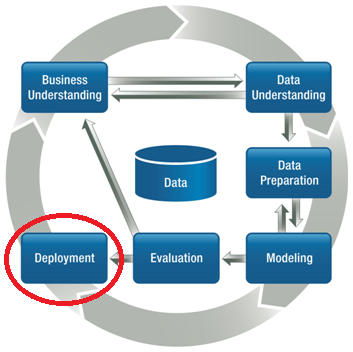
\includegraphics[width=0.5\textwidth]{./images/CRISPDM_6.png}
	\caption{CRISP-DM - Deployment}
	\label{CRISPDM_6}
\end{figure}
\section{Piano di Deployment}
The objective now is to put into action the commitments made in the opening step, according to the (presumably) new, valid, and operational information from the previous process steps.
The assimilation of knowledge demands for the formulation of ways in which the new information can be best exploited.
The specific business actions to be taken depend on the kind of application being developed and the executive commitments in the opening step.


Il filtro anti spam creato, visti i risultati positivi ottenuti, può essere utilizzato come ulteriore filtro ai già presenti filtri integrati nei principali gestori di posta elettronica, quali outlook e thunderbird.
\section{Monitoraggio e Manutenzione}
Careful preparation of a maintenance strategy helps to
avoid unnecessarily long periods of incorrect usage of
data mining results.
OUTPUT:
A maintenance plan on the monitoring process.
\section{Report Finali}
At the end of the project it is better to write up a final
report, which can be:
\begin{itemize}
	\item A summary of the project
	\item A final presentation of the data mining results
\end{itemize}
OUTPUT:
A report or a final presentation or both
\section{Revisione del lavoro}
Experience documentation help to consolidate important
experiences made for future engagements. The documentation
may include:
\begin{itemize}
	\item pitfalls
	\item misleading approaches
	\item hints for selecting the best-suited data mining technique in similar situations.
\end{itemize}
